\secnumbersection{VALIDACIÓN DE LA SOLUCIÓN}

Se debe validar la solución propuesta. Esto significa probar o demostrar que la solución propuesta es válida para el entorno donde fue planteada.

Tradicionalmente es una etapa crítica, pues debe comprobarse por algún medio que vuestra propuesta es básicamente válida. En el caso de un desarrollo de software es la construcción y sus pruebas; en el caso de propuestas de modelos, guías o metodologías podrían ser desde la aplicación a un caso real hasta encuestas o entrevistas con especialistas; en el caso de mejoras de procesos u optimizaciones, podría ser comparar la situación actual (previa a la memoria) con la situación final (cuando la memoria está ya implementada) en base a un conjunto cuantitativo de indicadores o criterios.

\subsection{EJEMPLO DE COMO CITAR TABLAS}

Se colocó una tabla que se puede referenciar también desde el texto (Ver tabla \ref{table:coloquios}).

\begin{table}[h]
    \centering
    \caption{\label{table:coloquios} Coloquios del Ciclo de Charlas Informática.} Fuente: Elaboración Propia.
    \begin{tabular}{|p{7cm}|p{7cm}|}
        \hline
        Título Coloquio & Presentador, País \\
        \hline
        ``Sensible, invisible, sometimes tolerant, heterogeneous, decentralized and interoperable... and we still need to assure its quality...''' & Guilherme Horta Travassos, Brasil.\\
        \hline
        ``Dispersed Multiphase Flow Modeling: From Environmental to Industrial Applications''' & Orlando Ayala, EE.UU.\\
        \hline
        ``Líneas de Producto Software Dinámicas para Sistemas atentos el Contexto''' & Rafael Capilla, España.\\
        \hline
        ... & ... \\
        \hline
    \end{tabular}
\end{table}

En la presente sección se presentarán las pruebas que validan los requerimientos de las herramientas/funcionalidades desarrolladas para las distintas aplicaciones de WiseConn.

\subsubsection{CONFIGURADOR DE MAPA}


\subsubsection{ALINEADOR DE IMÁGENES}

Esta funcionalidad se encuentra en la sección de proveedores externos en la herramienta de Admin de Dropcontrol. Para acceder 

\subsubsection{GRAFICADOR LIBRE}

Esta nueva herramienta implementada en la aplicación de \textit{Admin de DropControl} se encuentra en el menú lateral como muestra en la figura \ref{fig:menu-admin-graf}

\begin{figure}[H]
	\centering
	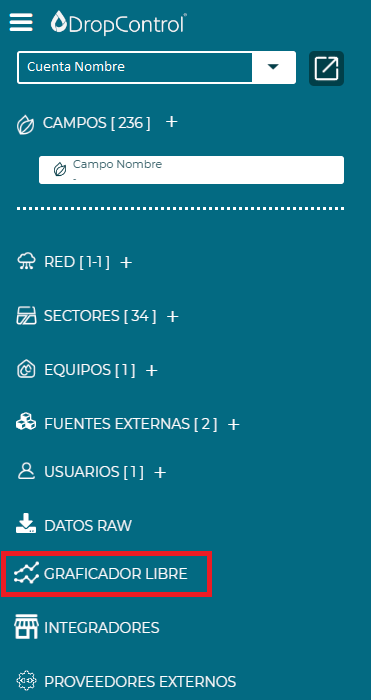
\includegraphics[width=0.5\textwidth]{menu-admin-graficador}
	\caption{\label{fig:menu-admin-graf} Graficador Libre en el menú de \textit{Admin}}
\end{figure}

En la herramienta se encontrará con 4 secciones, como se muestra en la figura \ref{fig:graf1}:
\begin{enumerate}
    \item Selección de nodo/sensores.
    \item Selección de rango de fechas.
    \item Gráfico.
    \item Tabla de datos.
\end{enumerate}

\begin{figure}[H]
	\centering
	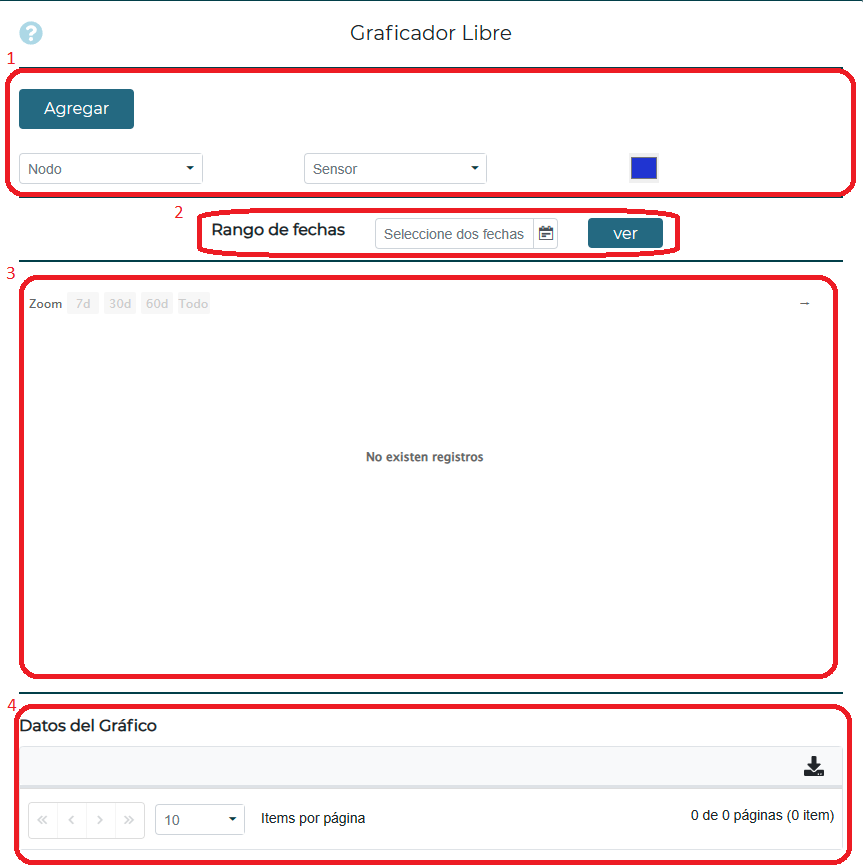
\includegraphics[width=0.8\textwidth]{graficador-1}
	\caption{\label{fig:graf1} Secciones del graficador libre}
\end{figure}

El primer paso es escoger los sensores que queremos visualizar en el gráfico, en la primera sección selecciones en el primer selector el nodo seguido del sensor y opcionalmente el color (Figura \ref{fig:grafselect}).

\begin{figure}[H]
	\centering
	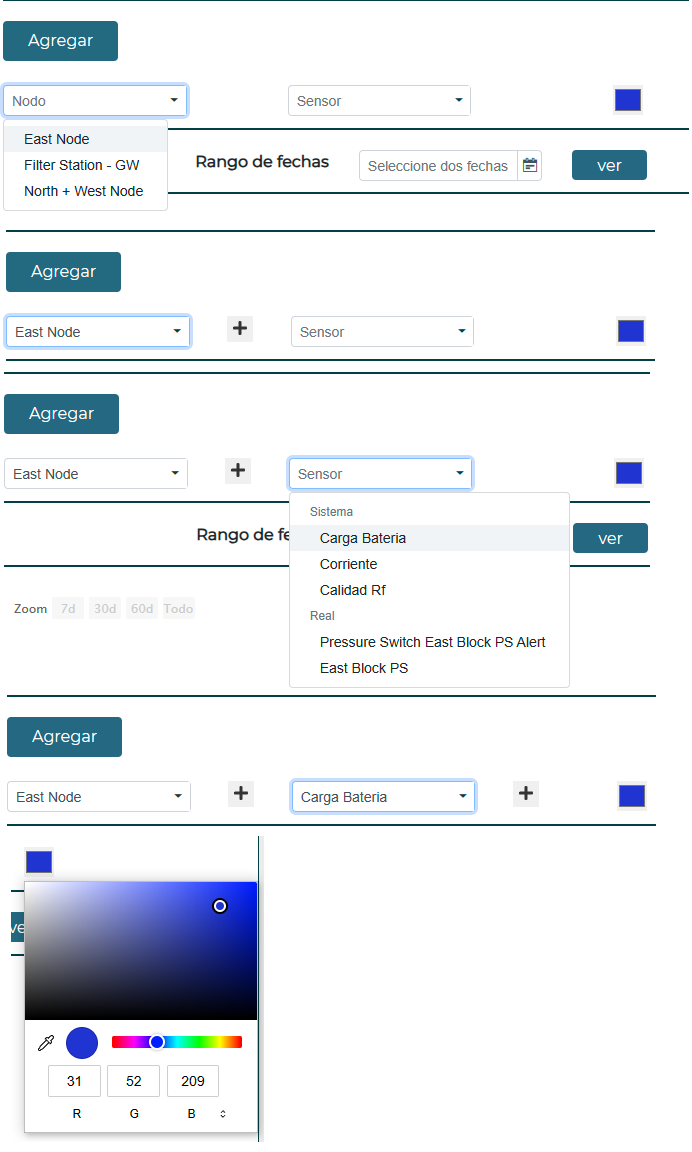
\includegraphics[width=0.8\textwidth]{graf-select}
	\caption{\label{fig:grafselect} Selección de sensor}
\end{figure}

Para escoger otro sensor se puede hacer agregando otra fila vacía haciendo click en el botón 'Agregar' (Figura \ref{fig:graf-add-row-1}) y repitiendo el paso anterior.

\begin{figure}[H]
	\centering
	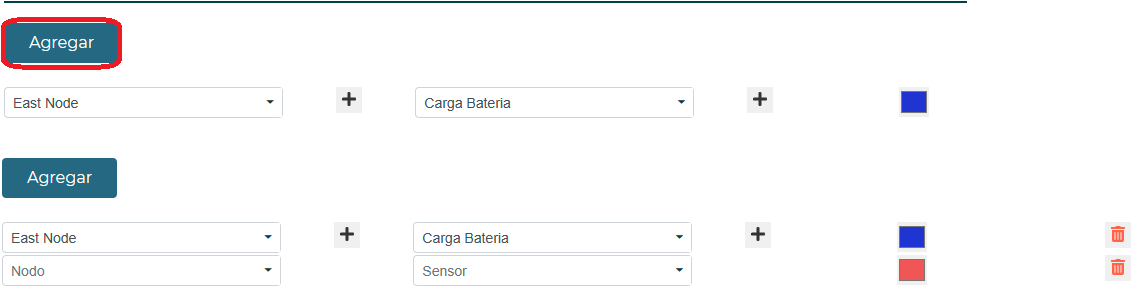
\includegraphics[width=0.8\textwidth]{graf-add-row-1}
	\caption{\label{fig:graf-add-row-1} Agregar una nueva fila vacía}
\end{figure}

Otra forma de agregar sensores es con los botones con el símbolo '+' presente en las filas. El primer botón agrega una nueva fila con el siguiente nodo seleccionado junto al sensor del mismo tipo (Figura \ref{fig:graf-add-row-2}), mientras que el segundo botón agrega una nueva fila con el mismo nodo seleccionado pero con el siguiente sensor en la lista (Figura \ref{fig:graf-add-row-3}).

\begin{figure}[H]
	\centering
	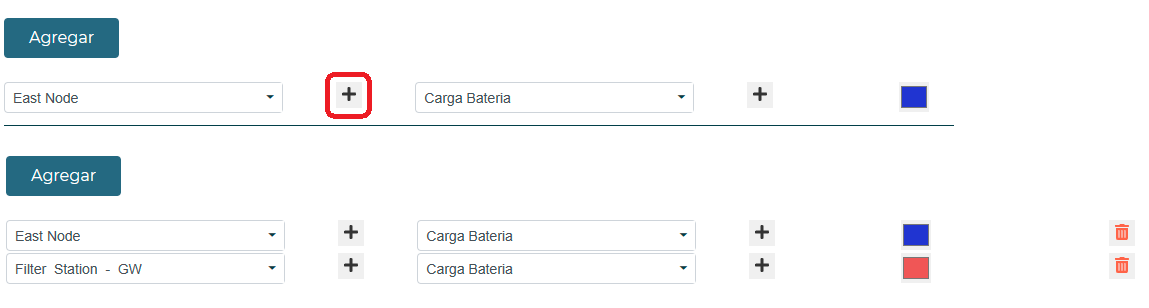
\includegraphics[width=0.8\textwidth]{graf-add-row-2}
	\caption{\label{fig:graf-add-row-2} Agregar una nueva fila con el siguiente nodo}
\end{figure}

\begin{figure}[H]
	\centering
	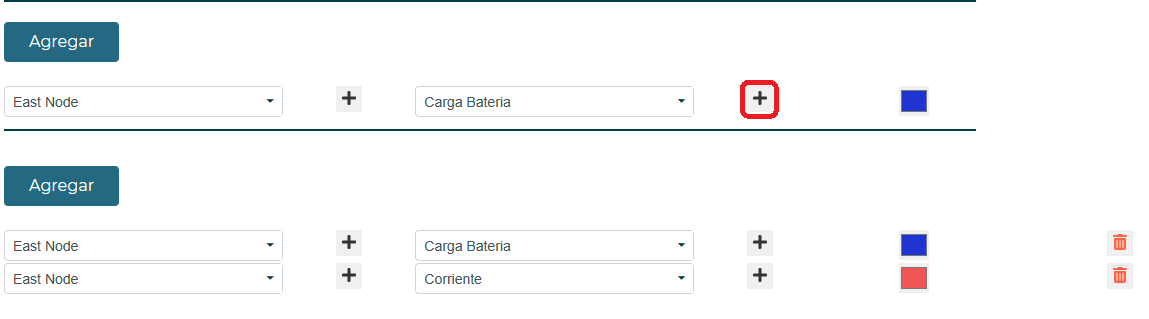
\includegraphics[width=0.8\textwidth]{graf-add-row-3}
	\caption{\label{fig:graf-add-row-3} Agregar una nueva fila con el siguiente sensor del nodo}
\end{figure}

Para eliminar una fila se debe hacer click en el último botón de la fila, con símbolo de basura (Figura \ref{fig:graf-delete-row}).

\begin{figure}[H]
	\centering
	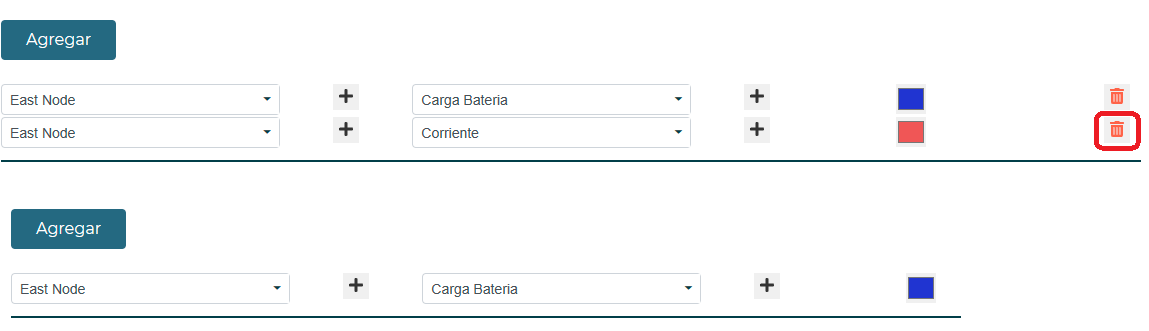
\includegraphics[width=0.8\textwidth]{graf-delete-row}
	\caption{\label{fig:graf-delete-row} Agregar una nueva fila con el siguiente sensor del nodo}
\end{figure}

El siguiente paso es escoger el rango de fechas de los datos, como se muestra en la figura \ref{fig:graf-date-range-1}.

\begin{figure}[H]
	\centering
	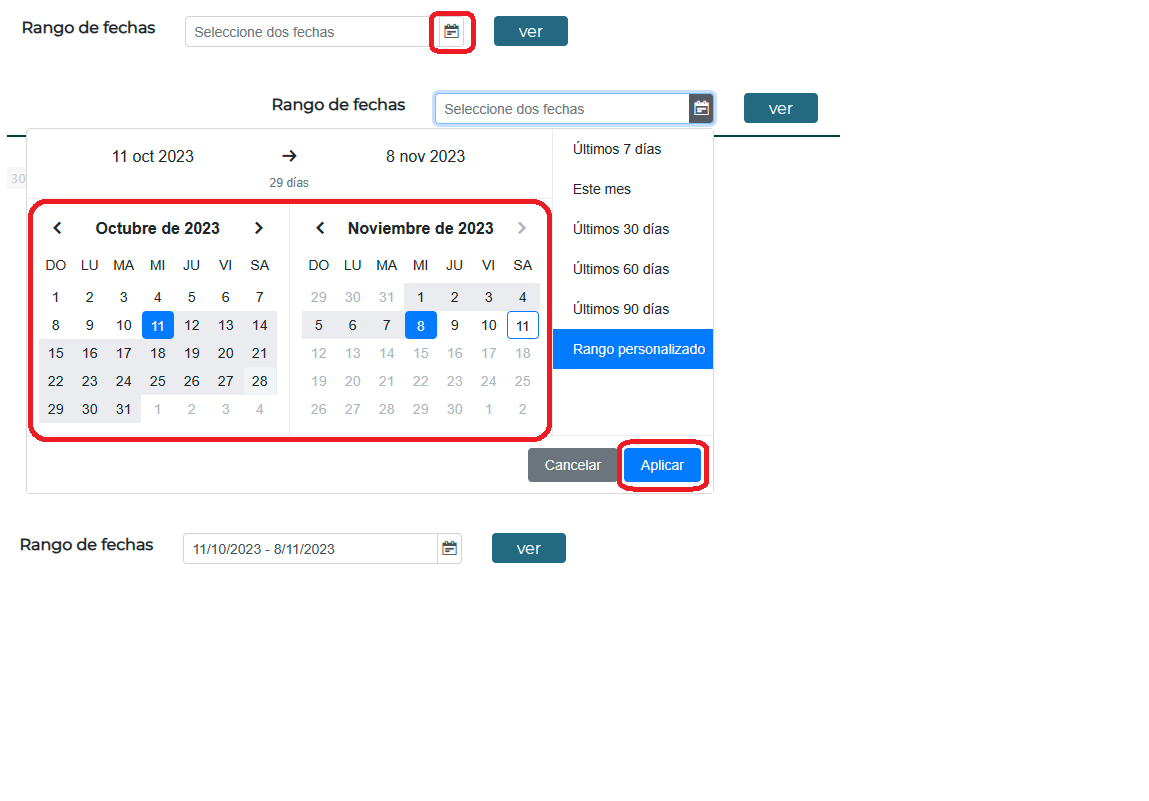
\includegraphics[width=0.8\textwidth]{graf-date-range-1}
	\caption{\label{fig:graf-date-range-1} Selección de rango de fechas}
\end{figure}

Se puede escoger un rango personalizado, como se mostró anteriormente, o escoger rangos predeterminados como muestra en la figura \ref{fig:graf-date-range-2}.

\begin{figure}[H]
	\centering
	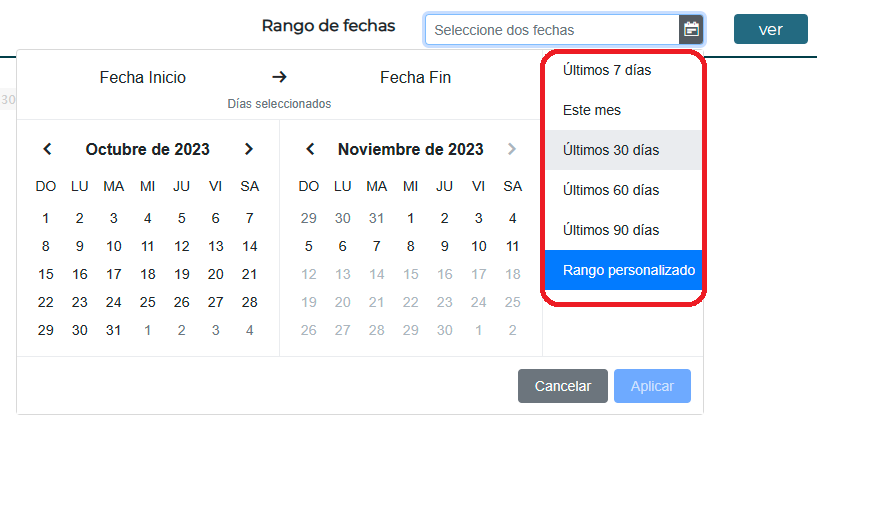
\includegraphics[width=0.8\textwidth]{graf-date-range-2}
	\caption{\label{fig:graf-date-range-2} Selección de rango de fechas}
\end{figure}

Luego de tener el rango de fechas seleccionado, hacer click en el botón 'ver' para mostrar los datos de los sensores seleccionados (Figura \ref{fig:graf-display-1})

\begin{figure}[H]
	\centering
	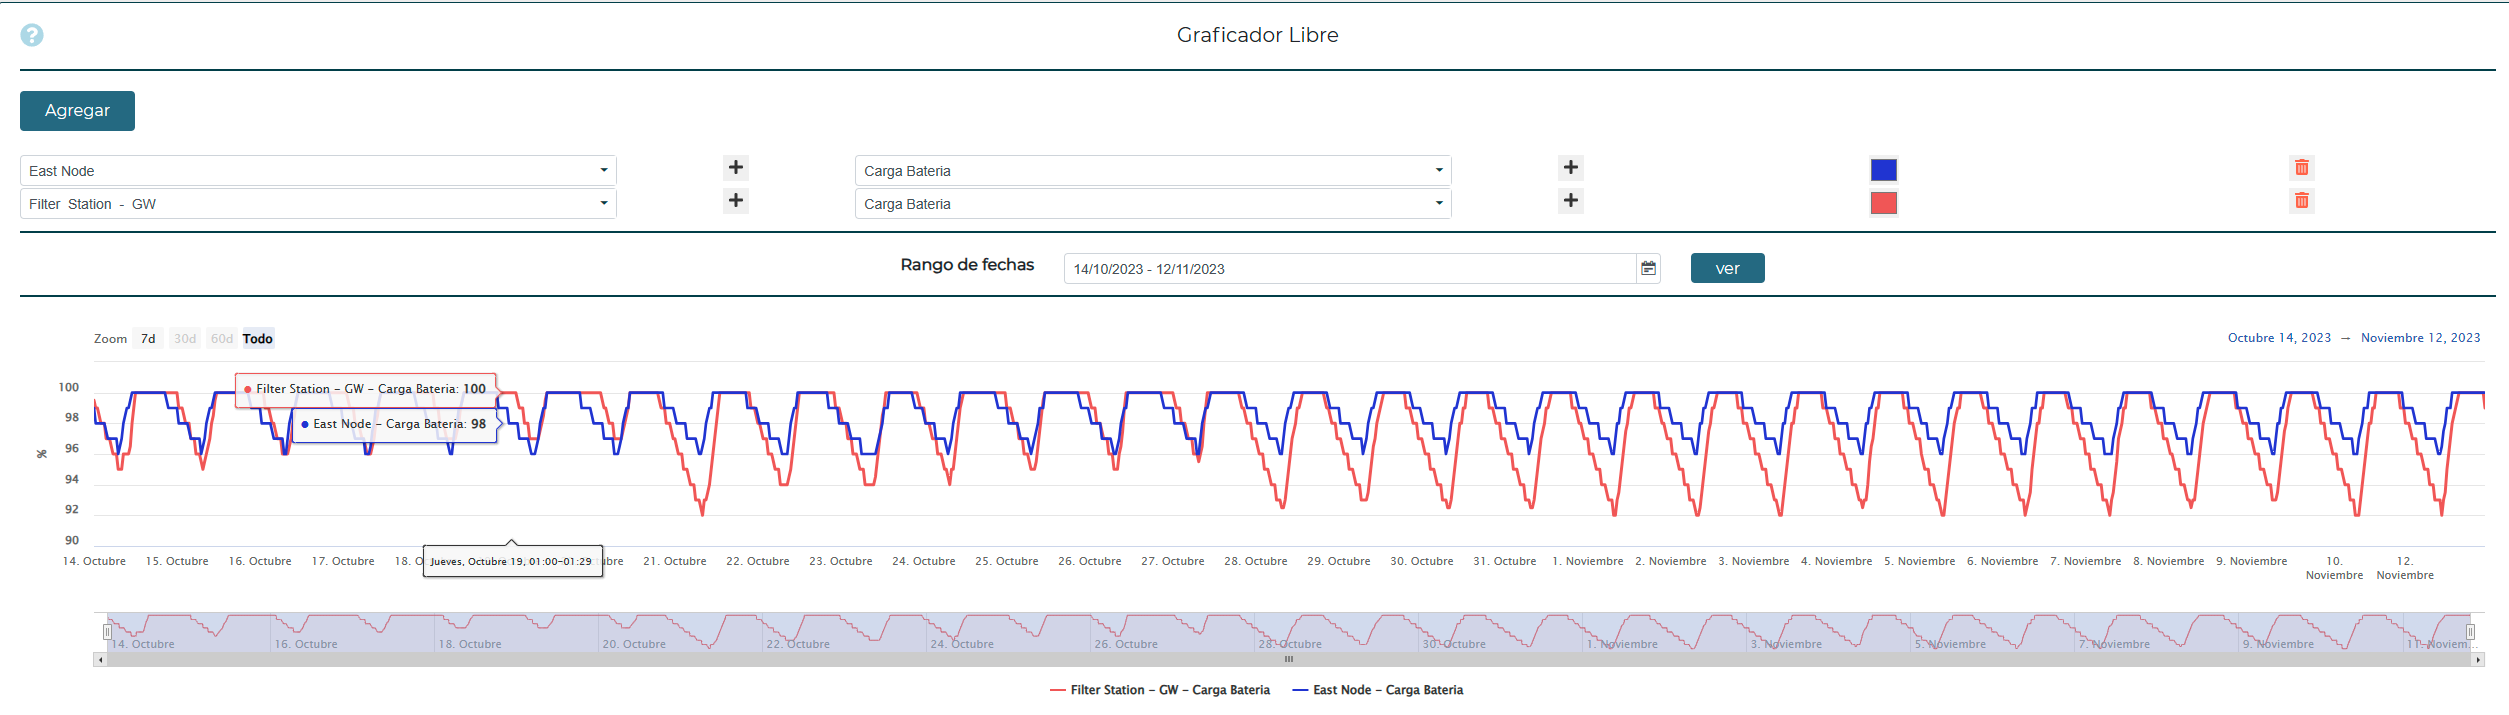
\includegraphics[width=0.8\textwidth]{graf-display-1}
	\caption{\label{fig:graf-display-1} Gráfico}
\end{figure}

En la última sección se encuentra la tabla de datos del gráfico, en donde se muestran los datos de los sensores donde la primera columna es la fecha y hora del dato y las columnas siguientes son los sensores escogidos con el formato de nombre \{Nodo\}-\{Sensor\} [unidad] (Figura \ref{fig:graf-table-1}). 
Además, tiene la funcionalidad de exportar la tabla en formato .xlsx haciendo click en el ícono de descarga en la esquina superior derecha de la tabla.

\begin{figure}[H]
	\centering
	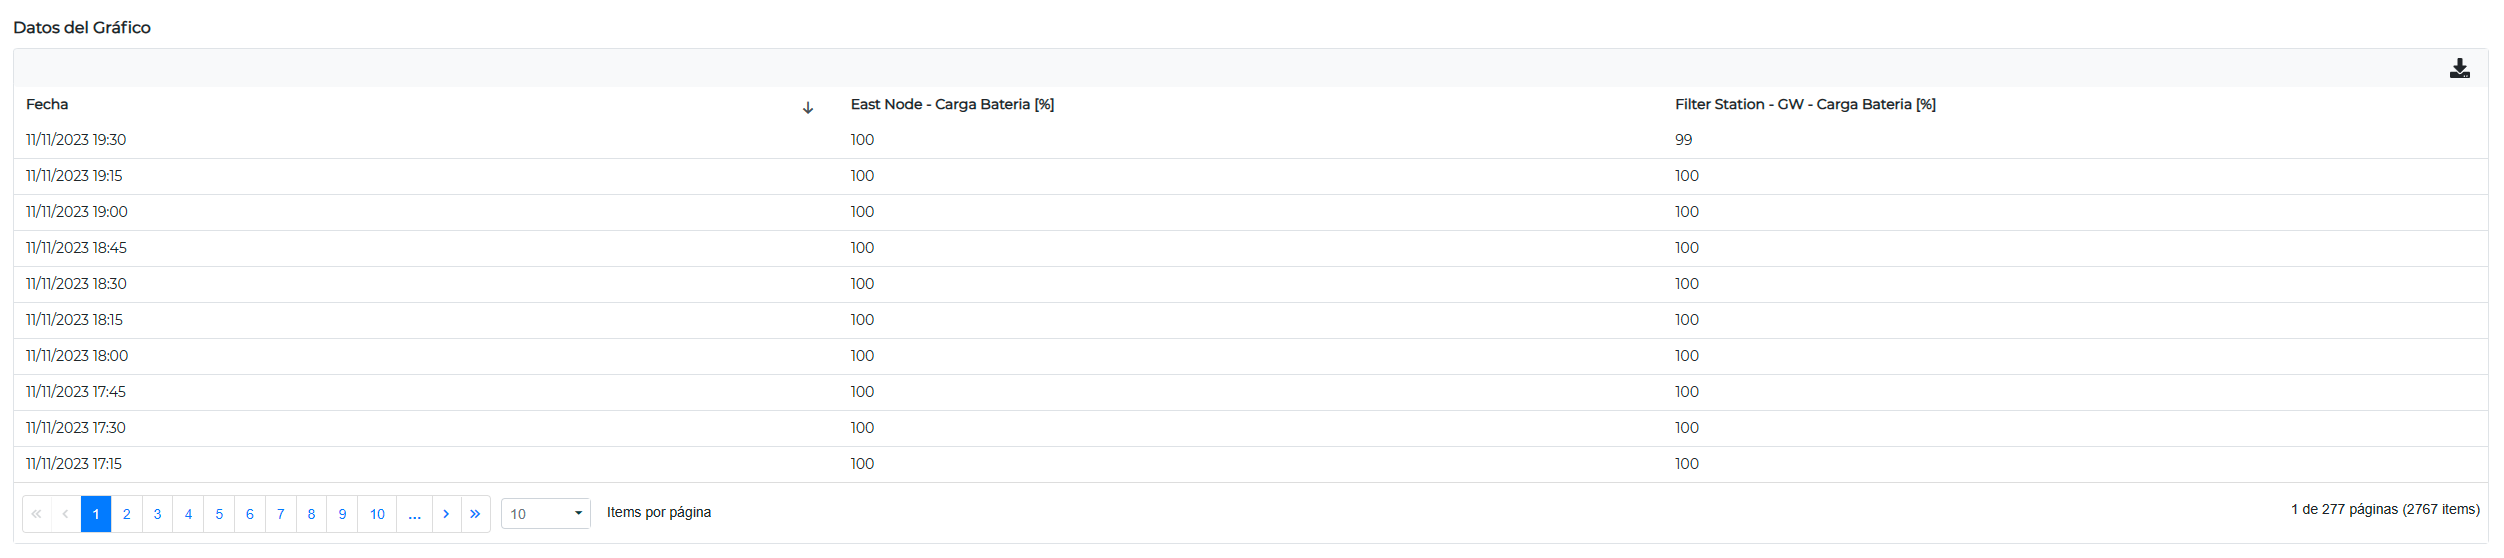
\includegraphics[width=0.8\textwidth]{graf-table-1}
	\caption{\label{fig:graf-table-1} Gráfico}
\end{figure}

\subsubsection{INTEGRADORES}

\subsubsection{CERTIFICADOS TESTBED}